\chapter{Кольори}\label{cha:color}
Найпоширенішим способом моделювання кольорів в комп'ютерній графіці є кольорова модель RGB, що відповідає способу відтворення кольору як на CRT-моніторах, так і на LCD-екранах / проекторах.

Кожен піксель представлений трьома значеннями - червоного, зеленого та синього каналів.

Таким чином, кольорове зображення у форматі RGB використовуватиме втричі більше пам'яті, ніж сіро-кольорове зображення з однаковими розмірами пікселів.

На рисунку 7 кольорове зображення, складене смугами червоного, зеленого та синього кольорів (це зображення ілюструє побудову дисплея ноутбука, зверніть увагу, що це зображення бажано переглядати на екрані комп'ютера, а не друкувати).

Одним з найпоширеніших форматів пікселів є 8 біт rgb, де значення червоного, зеленого та синього зберігаються з чергуванням у пам'яті.
Таке розташування пам'яті часто називають \textbf{кремезним(chunky)}, зберігання компонентів в окремих буферах називається \textbf{площинним(planar)}, і не так часто застосовується.

\begin{figure}
    \label{fig:image7}
    \centering
    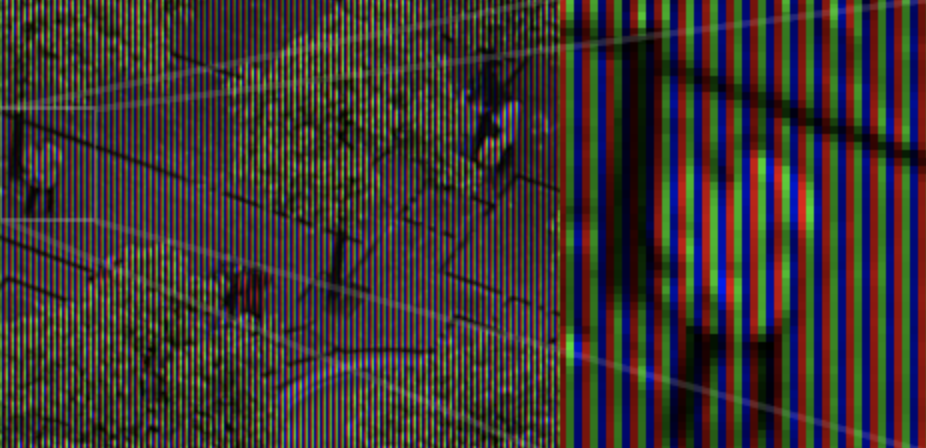
\includegraphics[scale=0.5]{image7.png}

    Рис. 7. Глибина зразка
\end{figure}


\section{Палітра / Індексовані зображення}\label{sec:palette}
Раніше було звичайним зберігати зображення в палетизованому режимі.
Ми зберігаємо лише номер запису палітри, що використовується для кожного пікселя.
І для кожного запису палітри ми зберігаємо кількість червоного, зеленого та синього світла.

На рисунку 8 зліва зображення використовує лише 16 кольорів, праворуч палітра, що використовується для цього зображення.
Принцип роботи індексованого / палітруваного зображення подібний до того, як працює фарба за номерами.

\begin{figure}
    \label{fig:image8}
    \centering
    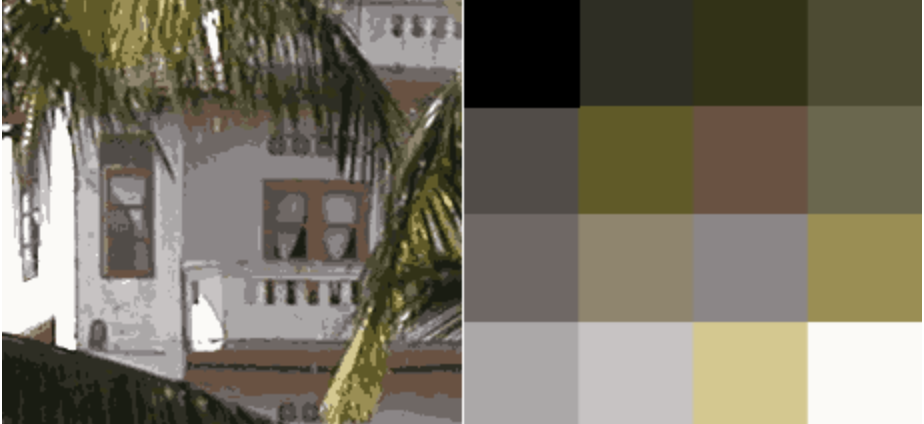
\includegraphics[scale=0.5]{image8.png}

    Рис. 8. Глибина зразка
\end{figure}


\section{Стиснення зображення.}\label{sec:image_compression}
Растрові зображення займають багато пам'яті, \textbf{стиснення зображення} зменшує обсяг пам'яті, необхідної для зберігання зображення.
Наприклад, 2,1-мегапіксельне 8-бітне RGB-зображення (1600x1200) займає 1600x1200x3 байт = 5760000 байт = 5,5 мегабайт, це нестиснутий розмір зображення.

\textbf{Коефіцієнт стиснення} - це співвідношення між стисненим зображенням і нестисненим зображенням, якщо згаданий вище приклад зображення зберігався як файл jpeg у розмірі 512 кб, коефіцієнт стиснення становив би 0,5 мб: 5,5 мб = 1:11.


\section{Стиснення зображення без втрат}\label{sec:lossless_image_compression}
Коли зображення стискається без втрат, повторення та передбачуваність використовуються для подання всієї інформації, використовуючи менше пам'яті.
Вихідне зображення можна відновити.
Одним з найпростіших методів стиснення зображень без втрат є кодування довжини циклу.
Кодування довжини циклу кодує послідовні та подібні значення, як один маркер у потоці даних.

На рисунку 9, “Кодування довжини циклу ”, чорно-біле зображення будинку було стиснене кодуванням довжини циклу, растрове зображення розглядається як один довгий рядок чорних / або білих пікселів, кодування - скільки байтів одного кольори виникають один за одним.
Ми ще більше зменшимо кількість байтів, зайнятих цими 72 числовими значеннями, маючи максимальну довжину інтервалу 15 і кодуючи довші інтервали за допомогою кількох інтервалів, розділених нульовими інтервалами іншого кольору.
\begin{figure}
    \label{fig:image9}
    \centering
    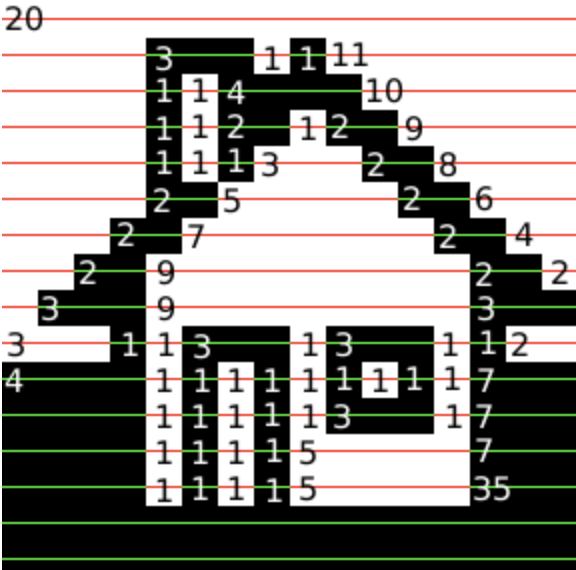
\includegraphics[scale=0.5]{image9.png}

    Рис. 9. Кодування довжини циклу (Run-length encoding)
\end{figure}

\begin{lstlisting}[style=light, language=Python,label={lst:vectorimg},caption=Кодування довжини циклу]
        70, 15, 0, 15, 0, 15, 0, 10,
         5, 25, 5, 15, 0, 10,
         5, 27, 6, 15, 0, 12,
         4, 26, 4, 15, 0, 11,
         4, 25, 4, 15, 0, 10,
         6, 24, 6, 15, 0, 9,
         6, 23, 6, 15, 0, 8,
         3, 2, 3, 22, 3, 2, 3, 15, 0, 7,
         3, 2, 3, 21, 3, 2, 3, 15, 0, 6,
         3, 5, 2, 20, 3, 5, 2, 15, 0, 5,
         3, 5, 2, 19, 3, 5, 2, 15, 0, 4,
         3, 7, 2, 18, 3, 7, 2, 15, 0, 3,
         3, 7, 2, 17, 3, 7, 2, 15, 0, 2
        14, 16, 14, 15, 0, 1
         3, 11, 2, 14, 3, 11, 2, 14,
         3, 11, 2, 13, 3, 11, 2, 13,
         3, 13, 2, 12, 3, 13, 2, 12,
         3, 13, 2, 11, 3, 13, 2, 11,
         3, 15, 2, 10, 3, 15, 2, 10,
         3, 15, 2, 8, 3, 15, 2, 8,
         6, 12, 6, 6, 6, 12, 6, 6,
         6, 12, 6, 64 6, 12, 6, 15, 0, 15, 0, 15, 0, 15, 0, 4
\end{lstlisting}


\section{Стиснення зображення з втратами}\label{sec:lossy_image_compression}
Стиснення з втратами використовує здатність людських очей приховувати недосконалість і той факт, що деякі типи інформації важливіші за інші.
Наприклад, зміни освітленості спостерігаються людиною як більш значущі, ніж зміна відтінку.

JPEG - це формат файлу, що реалізує стиснення на основі дискретного косинусного перетворення DCT, разом з алгоритмами без втрат, що забезпечує хороші коефіцієнти стиснення.
Спосіб роботи JPEG найкраще підходить для зображень із безперервними тональними діапазонами, таких як фотографії, логотипи, відсканований текст та інші зображення з безліччю чітких контурів / ліній, отримують більше артефактів стиснення, ніж фотографії.

\subsection{Втрати через покоління}\label{sec:loss_through_generations}
Алгоритми стиснення втрат не слід використовувати як робочий формат, лише кінцеві копії слід зберігати у форматі jpeg, оскільки втрати накопичуються протягом поколінь.

Зображення 10, спеціально побудоване для показу недоліків алгоритму стиснення JPEG, збережене, повторно відкрите та збережене знову 9 разів.

JPEG найбільш підходить для фотографічного вмісту, коли несприятливий ефект алгоритму стиснення не так очевидний.

JPEG не підходить як проміжний формат, використовуйте JPEG лише для остаточного розповсюдження, де розмір файлу насправді має значення.

\begin{figure}
    \label{fig:image10}
    \centering
    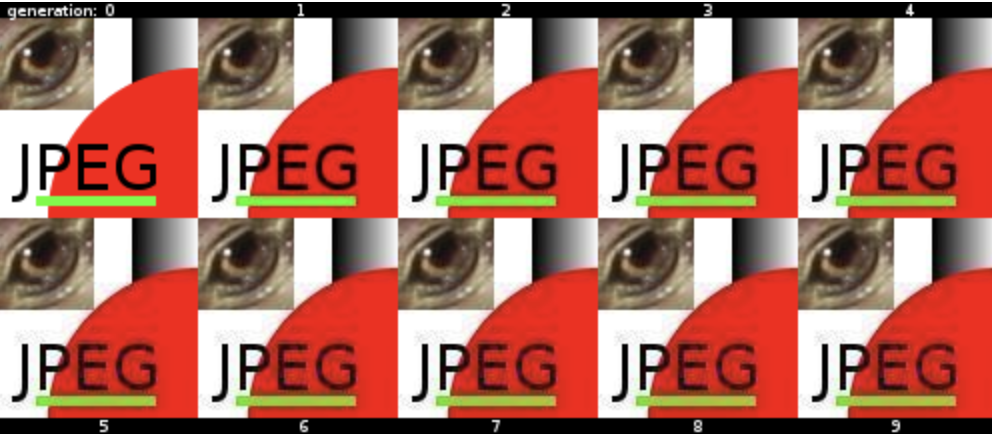
\includegraphics[scale=0.5]{image10.png}

    Рис. 10. Втрата якості через кілька генерацій JPEG
\end{figure}


\section{Формати файлів та програми}\label{sec:image_formats}
Багато програм мають власний внутрішній формат файлу, тоді як інші формати більше підходять для обміну даними.
У таблицях на малюнках 10 та 11 перелічено деякі поширені формати зображень.

\begin{figure}
    \label{fig:image11}
    \centering
    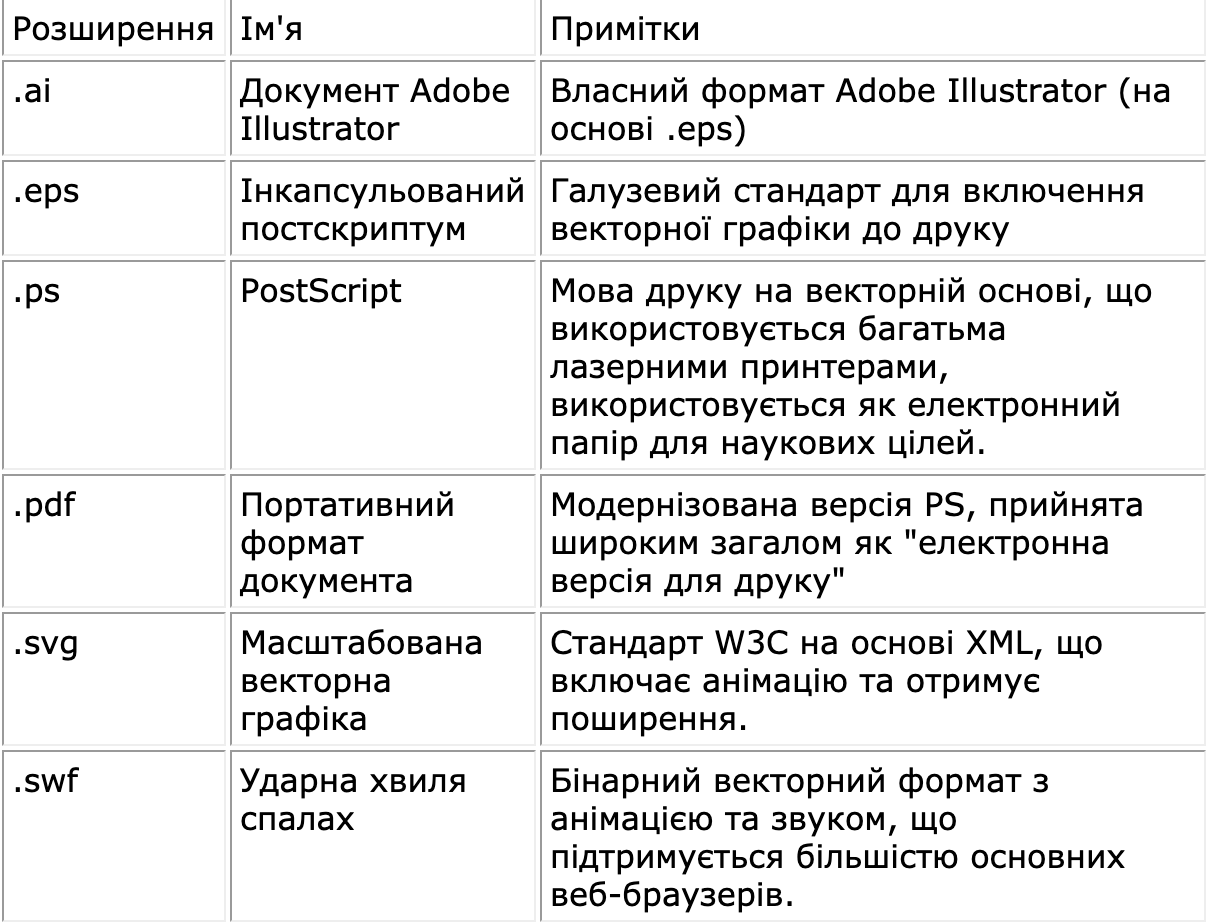
\includegraphics[scale=0.5]{image11.png}

    Рис. 11. Формати векторних файлів.
\end{figure}

\begin{figure}
    \label{fig:image12}
    \centering
    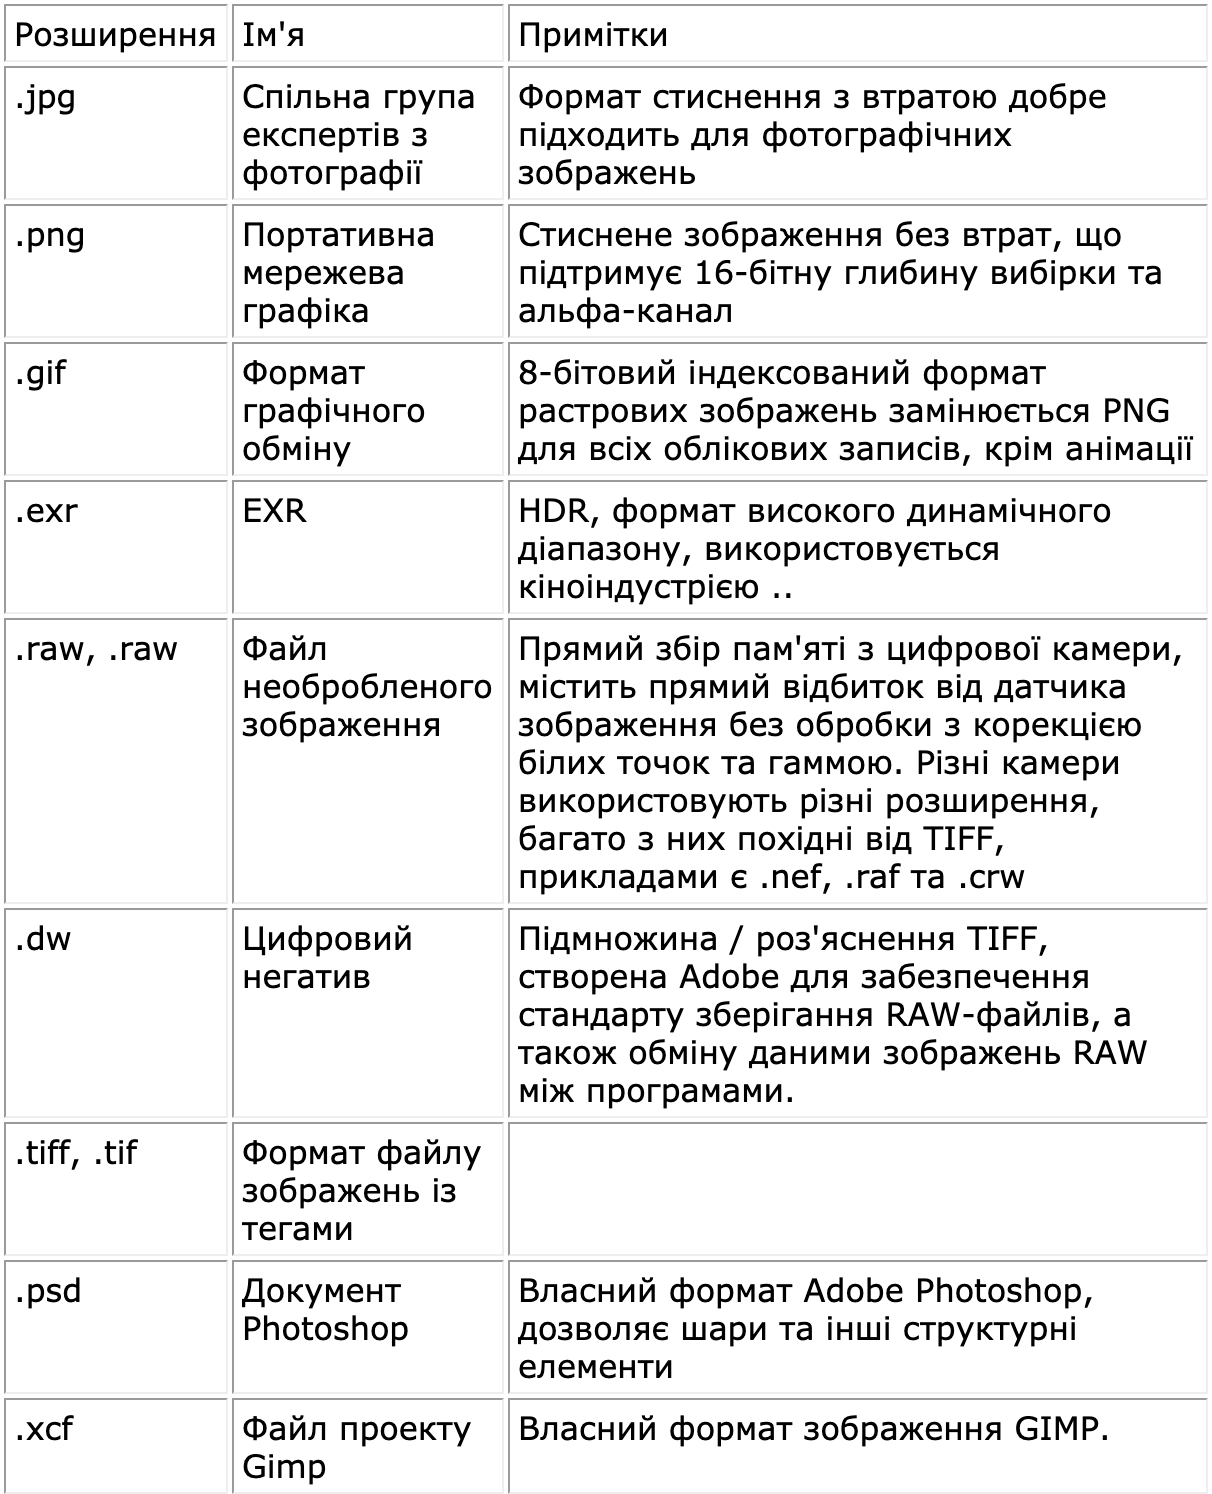
\includegraphics[scale=0.5]{image12.png}

    Рис. 12. Формати растрових файлів.
\end{figure}
